\section{Approach Design}
In this section, we give a detailed description of our approach, which targets on utilizing GPU to match query graphs on labeled graphs.
\subsection{Approach Overview}
Before the matching process, we first convert the data graph into our specific format that is space efficient and query friendly. Note that the conversion only needs to do once. Then, we perform subgraph matching on GPU, as shown in Algorithm \ref{algo:submatch}. We first decompose the query graph into query phases based on its vertex and edge labels. In the meanwhile, we generate a matching order for query phases and restrictions on query vertices (line 1). All edges extended in a query phase have the same edge label since we load one edge label partition at each iteration (lines 2, 7).
%\RV{There are two types of query phases, \emph{extension phase} that contains one of extension patterns 0-7 (line 9), and \emph{elimination phase}. We use SV-phase and NV-phase to represent extension phases that contain extension pattern 0 and extension patterns 1-7, respectively}.
The elimination phase contains multiple backward edges for elimination (line 11). The first query phase of the matching order is used to generate initial embeddings. We use the same GPU kernel as the extension phase to generate initial embeddings (line 4). The main difference between the first query phase and the extension phase is that the source VIDs of the former one are from the edge label partition, while the later one are from previous embeddings. Finally, we use different GPU kernels to match different types of query phases (lines 10, 12), and output the final embeddings (line 13). In the following sections, we elaborate each step in detail.

\begin{algorithm}[t!]
\KwIn{the data graph in our format $G$, the query graph $q$}
\KwOut{Embeddings of $q$ $EMB$}
$\pi \leftarrow \textsc{GenMatchOrder}(q)$\;
Load the edge label partition $elp$ whose edge label is $\pi[0].edgeLabel$ from $G$ to GPU\;
Allocate all available GPU memory space to $newEMB$\;
$\textsc{ExtKernel}(elp,NULL,newEMB,\pi[0])$\;
$EMB \leftarrow newEMB$\;
\For{$i \leftarrow 1$ \KwTo $\pi .size$}{
	Load the edge label partition $elp$ whose edge label is $\pi[i].edgeLabel$ from $G$ to GPU\;
	Allocate all available GPU memory space to $newEMB$\;
	\If{$\pi[i]$ is an extension phase}{
		$\textsc{ExtGPUKernel}(elp,EMB,newEMB,\pi[i])$\;
	}
	\Else{
		$\textsc{EliGPUKernel}(elp,EMB,newEMB,\pi[i])$\;
	}
	$EMB \leftarrow newEMB$\;
}
\caption{\textsc{SubgraphMatching}}
\label{algo:submatch}
\end{algorithm}


\subsection{Data Graph Format}
\begin{figure*}
\centering
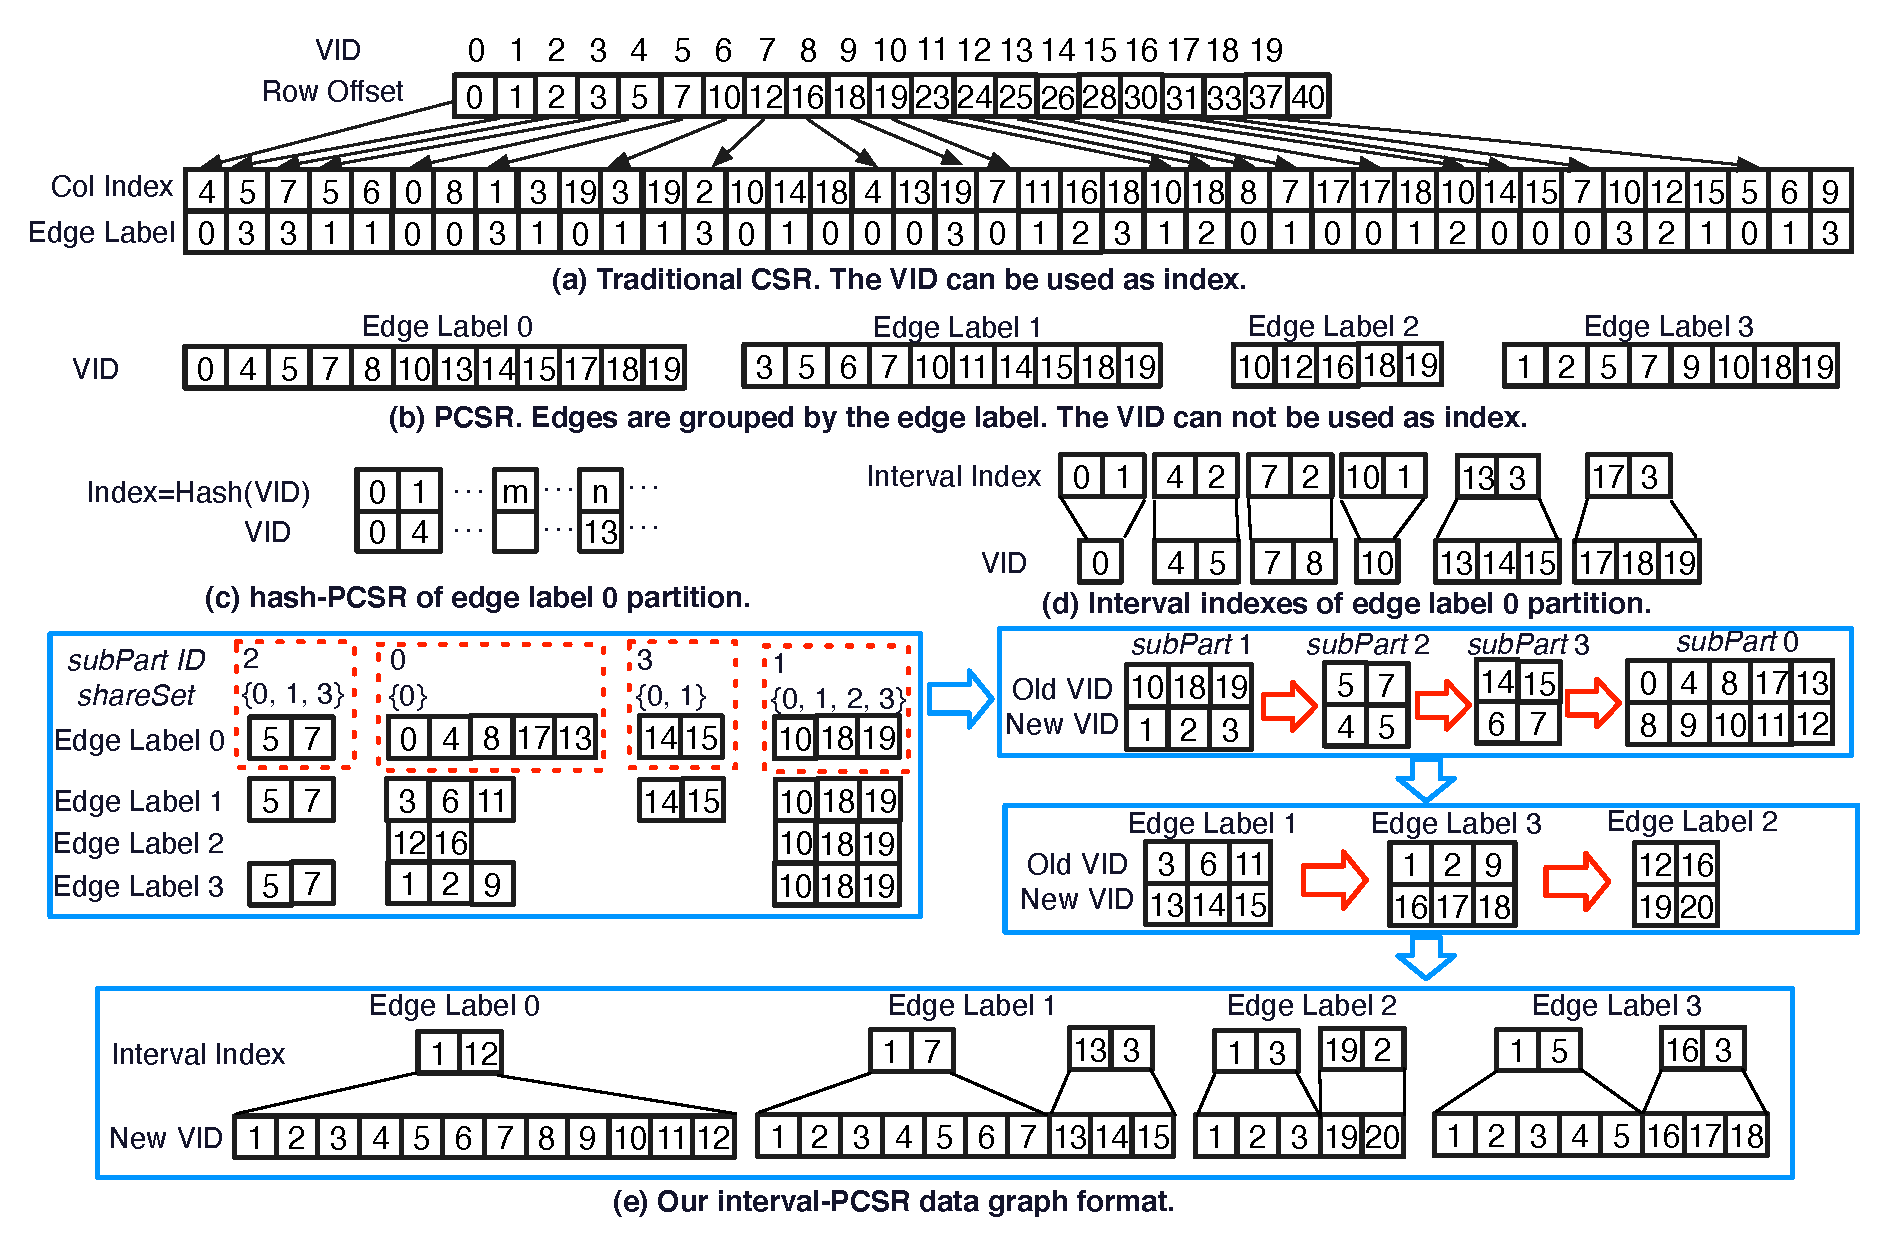
\includegraphics[width=\textwidth]{./figure/graphformat.eps}
\caption{Demonstration of data graph formats generated by traditional CSR, PCSR, hash-PCSR, non-optimized interval-PCSR, and our optimized interval-PCSR. Note that both non-optimized and optimized interval-PCSR do not need to store VIDs.}	
\label{fig:dataformat}
\end{figure*}

We first briefly describe the state-of-the-art data graph format for labeled graphs on GPU, hash-PCSR, which is proposed by GSI \cite{zeng2020gsi}. Then, we give a detailed illustration of our data graph format, interval-PCSR, which is more space and time efficient than hash-PCSR.
\subsubsection{hash-PCSR}
hash-PCSR groups edges of the same edge label into one edge label partition and builds the GPU-based CSR format for each edge label partition. Thus, only the partition that has the same edge label as the matching edge needs to be transferred to GPU memory, which significantly reduces the GPU memory consumption. In the traditional CSR format (Figure \ref{fig:dataformat}(a)), a VID can be used as the index to find the row offset of this vertex because VIDs in CSR are contiguous. However, VIDs may not be contiguous in an edge label partition (Figure \ref{fig:dataformat}(b)), and hence can not be used as the index. To overcome this problem, hash-PCSR designs a hash function to generate an index for each vertex based on its VID (Figure \ref{fig:dataformat}(c), this is a simplified hash-PCSR format, the detailed format is in \cite{zeng2020gsi}). To reduce collisions of the hash function, hash-PCSR uses 30 empty entries for each vertex and results in a large portion of unused GPU memory space.
\subsubsection{Our interval-PCSR}
\begin{algorithm}[t!]
\KwIn{the set of all edge label partitions $ELP$}
\KwOut{the mapping array $MAP$ with old and new vertex IDs are indices and values respectively}	
$newVID \leftarrow 1$\;
\While{ $ELP \neq \emptyset$ }{
	Choose the partition $elp \in ELP$ that has the most vertices\;
	Divide $elp$ into sub-partitions $subParts$\;
	\ForEach{$subPart \in subParts$}{
		Group IDs of partitions that contain $subPart$ into $shareSet$ and delete vertices of $subPart$ from these partitions\;
	}
	\While{$subParts \neq \emptyset$}{
		Choose the $subPart \in subParts$ that is shared by the most partitions and delete it from $subParts$\;
		Construct $MAP$ (assign new vertex IDs starting from $newVID$ to vertices in $subPart$ contiguously)\;
		$newVID \leftarrow newVID + subPart.size$\;
		$preSubPart \leftarrow subPart$\;
		\While{$preSubPart \neq \emptyset$}{
			Choose the $subPart \in subParts$ whose $shareSet$ has the most same partition IDs with the $shareSet$ of $preSubPart$ and delete the $subPart$ from $subParts$\;
			\If{Found the $subPart$}{
				Construct $MAP$\;
				$newVID \leftarrow newVID + subPart.size$\;
				$preSubPart \leftarrow subPart$\;
			}
			\Else{
				$preSubPart \leftarrow \emptyset$\;
				break\;
			}
		}
	}
	$ELP \leftarrow ELP/elp$\;
}
\caption{\textsc{GenMap}}
\label{algo:genmap}
\end{algorithm}

Our data graph format utilizes PCSR as the underlying data graph format but possesses efficient memory usage. To reduce the amount of unused memory space caused by the hash function, we leverage the interval index to represent contiguous VIDs in an edge label partition, as shown in Figure \ref{fig:dataformat}(d). Each interval index needs two entries to store the first VID and the length of this interval. The main issue of interval index format is that an edge label partition may contain numerous small intervals, which causes a number of memory accesses to find the right interval for a VID. For example, if we want to find the index of VID 7 in Figure \ref{fig:dataformat}(d), we need to compare 7 with the first three interval indexes and find VID 7 in the third interval index. With careful design, we can compare VID 7 only once to find its index. The key idea of our interval-PCSR is to design a mapping from original VIDs to new VIDs, which can generate more contiguous new VIDs in each edge label partition. Figure \ref{fig:dataformat}(e) and Algorithm \ref{algo:genmap} describe the workflow of our VID mapping process. The core design of our VID mapping algorithm can be explained by answering three questions:
\begin{itemize}
  \item[\emph{Q1:}] \emph{How to decide which partition should be assigned with new contiguous VIDs first?}\\We choose the partition that contains the most vertices (line 3) because the more vertices it contains, the higher probability it will be accessed. Therefore, reducing the number of intervals for this partition can help reduce the memory access latency. Figure \ref{fig:dataformat}(e) shows that edge label partition 0 is selected because it contains the most vertices.
  \item[\emph{Q2:}] \emph{How to decide which vertices of the partition should be assigned with new contiguous VIDs first?}\\We first group vertices shared by the same partitions into the same sub-partitions (line 4). After that, we only need to choose the best suitable sub-partition instead of vertices because vertices in a sub-partition can be assigned in any order without affecting the final interval index. For example, the edge label partition 0 in Figure \ref{fig:dataformat}(e) is divided into four sub-partitions. For $subPart$ 1, we can also map old VIDs 10, 18, and 19 to 2, 3, and 1, respectively, and the final interval index will still be the same. Then, we choose the sub-partition shared by the most partitions and assign its vertices with new VIDs contiguously (lines 8-10). The reason is that this kind of sub-partition has the most relations with other sub-partitions, and thus we try to assign contiguous VIDs to vertices in these related sub-partitions to reduce the total number of intervals. For example, in Figure \ref{fig:dataformat}(e), $subParts$ 1 and 2 are the most related sub-partitions. Thus we assign vertices in both sub-partitions contiguously, and all edge label partitions that contain both sub-partitions can represent them with one interval index.
  \item[\emph{Q3:}] \emph{How to decide which sub-partition should be processed next?}\\One or more partitions share the same sub-partition, and we call these partitions the $shareSet$ of the sub-partition (line 6). We intersect the $shareSet$ of each sub-partition with that of the previously selected sub-partition, and choose the sub-partition that has the largest intersection set (lines 13-20). In this way, we can assign contiguous VIDs to sub-partitions that exist in most partitions to reduce the number of interval indexes.
\end{itemize}

After replacing old VIDs with new VIDs, we build interval indexes, row offset, and column indexes for each edge label partition. Additionally, we group neighbors of each vertex by vertex labels and then sort neighbors in each group by their VIDs. To speed up the searching process of a VID, we load interval indexes of an edge label partition into GPU shared memory. In summary, our interval-PCSR is more space efficient than hash-PCSR in two aspects: (1) interval-PCSR does not need to store VIDs while hash-PCSR needs VIDs to evaluate whether the VID pointed by the hash index is the searching VID; (2) interval-PCSR has no empty entries while hash-PCSR uses 30 empty entries for each vertex to reduce collisions of the hash function.


\subsection{Extension Phase}
\begin{figure}
\centering
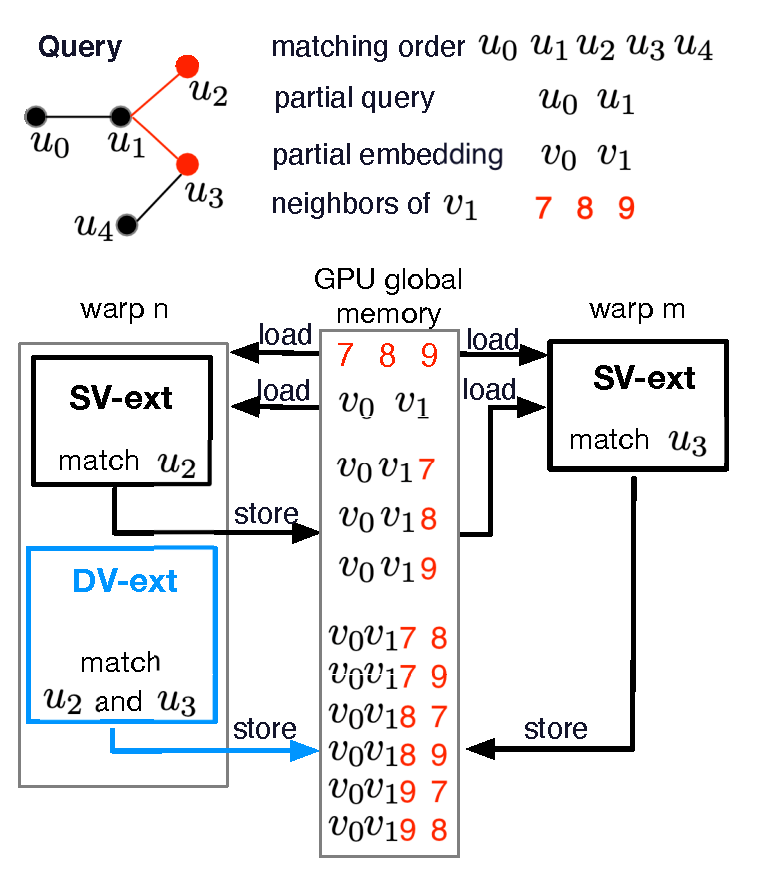
\includegraphics[width=0.9\columnwidth]{./figure/doubleext.eps}
\caption{Examples of single-vertex extension and our N-vertex extension methods.}	
\label{fig:doubleext}
\end{figure}
Previous works \cite{zeng2020gsi,sun2020subgraph} adopt the traditional single-vertex extension (SV-ext) method when matching the query graph in a data graph. However, this method ignores some critical information of the query graph when extending partial embeddings. In Figure \ref{fig:doubleext}, the SV-ext method needs to write intermediate results after matching $u_2$ and read intermediate results before matching $u_3$. This procedure is time-consuming because both write and read operations need to access GPU global memory. In order to speed up the matching process, \RV{we propose N-vertex extension (NV-ext) method that can extend partial embeddings with as many vertices as possible in one step. Our NV-ext method can handle all extension patterns shown in Figure \ref{fig:extpattern}}.


The main problem of subgraph matching on GPU is that the number of partial embeddings generated by each warp is different, thus we need to find the write address of new partial embeddings for each warp to avoid write conflicts. To solve this problem, GSI \cite{zeng2020gsi} uses a Prealloc-Combine method, which needs two extra GPU kernels and access all partial embeddings twice to find the write address for each warp. Though Prealloc-Combine method is more efficient than GpSM \cite{tran2015fast} which generates partial embeddings twice, it still incurs high memory overhead. Different from GSI, we use $atomicAdd$ inside the GPU kernel to calculate write addresses. The main performance issue of $atomicAdd$ is the sequential execution when multiple warps update the same variable at the same time. But this is not a severe problem in subgraph matching because of the intrinsic irregularity of subgraph matching.

We now explain how to generate partial embeddings for these four extension patterns, as illustrated in Algorithm \ref{algo:extphase}. For each partial embedding (line 3), we first get source VIDs from the partial embedding according to the extension phase (line 4). Then, we search source VIDs in interval indexes and extract their neighbors (line 5).  Next, we remove invalid neighbors that have wrong vertex labels and do not satisfy restrictions. Finally, we use different algorithms to generate new embeddings for different extension patterns (lines 8-13).

\begin{algorithm}
\KwIn{the edge label partition $elp$, partial embeddings $EMB$, the starting address of new embeddings $newEMB$, the extension phase $extPhase$}
$count \leftarrow 0$\;
Load interval indexes of $elp$ into shared memory\;
\ForEach{$emb \in EMB$}{
	\tcp{For EPs 1 and 3, $u_{s1}=u_{s2}$}
	Get source VIDs $u_{s1}$ and $u_{s2}$ from $emb$ according to $extPhase$\;
	Search $u_{s1}$ and $u_{s2}$ in interval indexes and extract their neighbors $ne1$ and $ne2$, respectively.\;
	Remove neighbors that do not have the same vertex labels as $u_{1}$ and $u_{2}$ from $ne1$ and $ne2$, respectively\;
	Remove neighbors that do not satisfy the restrictions of $u_{1}$ and $u_{2}$ from $ne1$ and $ne2$, respectively\;
	\If{$extPhase$ is EP 1}{
		$\textsc{OptDouExt}(emb,ne1,count,newEMB)$\;
	}
	\ElseIf{$extPhase$ is one of EPs 2, 3, and 4}{
		$\textsc{DouExt}(emb,ne1,ne2,count,newEMB)$\;
	}
	\Else{
		This is an extension phase that contains one vertex. We use the traditional method to generate embeddings for $extPhase$\;
	}
}

\caption{\textsc{ExtPhaseKernel}}
\label{algo:extphase}
\end{algorithm}

For extension patterns 2-4, we devise a direct method, Algorithm \ref{algo:generalDV}, to generate new embeddings. The main idea of Algorithm \ref{algo:generalDV} is to iterate over all combinations of candidates of $u_{1}$ and $u_{2}$, denoted as $C_1$ and $C_2$ respectively, and construct new embeddings by appending each valid combination to a new copy of the current embedding $emb$. We say a combination is valid, if neither VIDs in the combination equals to VIDs in $emb$. To avoid checking this condition repeatedly, we first check this condition for all vertices in $C_2$ once (lines 3-4) and record indexes of vertices whose VIDs also exist in $emb$ (line 5). To fully utilize $C_2$, we generate new embeddings while checking the condition. Once a vertex in $C_2$ is checked valid (lines 6-7), we assign this vertex and the first valid vertex in $C_1$ to $u_2$ and $u_1$, respectively (lines 1,8). Then, we write the new partial embedding $(emb,u_1,u_2)$ to the corresponding address (lines 9-10).

\begin{algorithm}
	\KwIn{the partial embedding $emb$, candidates of $u_1$ $C_1$, candidates of $u_2$ $C_2$, the number of newly written embeddings $totNum$, the starting address of new embeddings $newEMB$}
	Find the index $i$ of the first valid vertex in $ne1$\;
	$writePos \leftarrow atomicAdd(totNum,1 \times C_{2}.size)$\;
	\For{$j \leftarrow 0$ \KwTo $C_{2}.size$}{
		\If{$C_2[j] \in emb$}{
			Add $j$ to the set $boundry$\;
			$u_1 \leftarrow 0$; $u_2 \leftarrow 0$\;
		}
		\Else{
			$u_1 \leftarrow C_1[i]$; $u_2 \leftarrow C_2[j]$\;
		}
		Write the new embedding ($emb$, $u_1$, $u_2$) to the address pointed by $newEMB+writePos$\;
		$writePos \leftarrow writePos + emb.size+2$\;
	}
	$i \leftarrow i+1$\;
	\While{$i < C_{1}.size$}{
		Load 32 candidates from $C_1$ into $tmp$; $i \leftarrow i+32$\;
		Remove candidates that exist in $emb$ from $tmp$\;
		$writePos \leftarrow atomicAdd(totNum,tmp.size \times (C_{2}.size-boundry.size))$\;
		\ForEach{$0 \leq k<tmp.size$ and $0 \leq j<C_{2}.size$ and $j \notin boundry$}{
			\If{This is EP 2 and $C_1[k]=C_2[j]$}{
				$u_1 \leftarrow 0$; $u_2 \leftarrow 0$\;
			}
			\Else{
				$u_1 \leftarrow C_1[k]$; $u_2 \leftarrow C_2[j]$\;
			}
			Write the new embedding ($emb$, $u_1$, $u_2$) to the address pointed by $newEMB+writePos$\;
			$writePos \leftarrow writePos + emb.size+2$\;
		}
	}
	\caption{\textsc{DouExt}}
	\label{algo:generalDV}
\end{algorithm}

At the beginning of Algorithm \ref{algo:generalDV}, we allocate space for new partial embeddings generated when checking conditions for $C_2$ (line 2). Since we do not know the number of valid vertices in $C_2$ until all vertices are checked, we use the vertex count of $C_2$, denoted as $C_{2}.size$, to overestimate the number of new partial embeddings. If there are invalid vertices in $C_2$, we assign 0 to $u_1$ and $u_2$ to indicate invalid partial embeddings (line 6). When a GPU kernel read a partial embedding that contains 0, it skips this partial embedding.

In Algorithm \ref{algo:generalDV}, after finding invalid vertices in $C_2$, we generate new partial embeddings for rest vertices in $C_1$ (lines 11-12). In each iteration, we load 32 vertices in $C_1$ into shared memory $tmp$ and remove invalid ones from $tmp$ (lines 13-14). In order to allocate space for new partial embeddings, we estimate its count as the number of combinations of $tmp$ and valid vertices in $C_2$ (line 15). Then, we generate new partial embeddings for these combinations (line 16). As $u_1$ and $u_2$ have the same vertex label in extension pattern 2, there is a chance that two candidates of $u_1$ and $u_2$ are equal (line 17), which makes the generated partial embedding invalid. Next, we assign 0 to $u_1$ and $u_2$ if the partial embedding is invalid (line18), otherwise assign corresponding candidates to $u_1$ and $u_2$ (line 20). Finally, write the new partial embedding to the specified address (lines 21-22).

However, Algorithm \ref{algo:generalDV} is not appropriate for extension pattern 1. In extension pattern 1, $u_1$ and $u_2$ are extended from the same source vertex $u_{s1}$ and have the same vertex label, thus $C_1 = C_2$. If Algorithm \ref{algo:generalDV} is applied to extension pattern 1, each vertex in $C_2$ can be accessed by up to $C_1.size$ times. As shown in the left part of Figure \ref{fig:ep1opt}, element 1 is accessed at each iteration of $i$. If $C_1.size>32$, we need to reload element 1 from global memory each time we access it. Other elements also encounter the same problem.

\begin{figure}
\centering
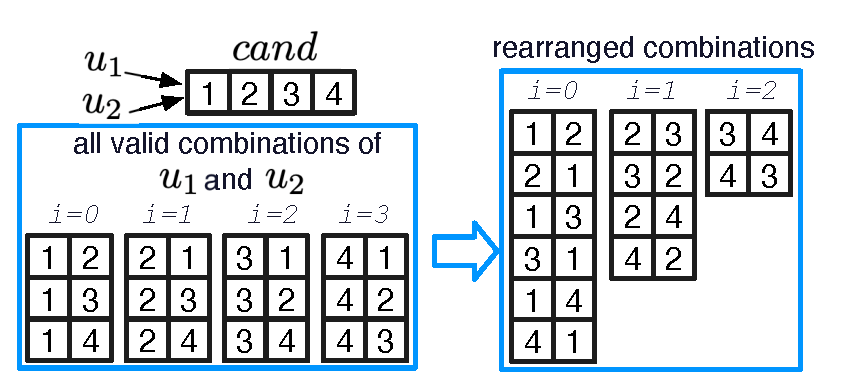
\includegraphics[width=\columnwidth]{./figure/ep1opt.eps}
\caption{An example of generating new embeddings for extension pattern 1.}	
\label{fig:ep1opt}
\end{figure}

To speed up the matching process of extension pattern 1, we rearrange the generation order of combinations, as shown in the right part of Figure \ref{fig:ep1opt}, to make accesses more register friendly. Algorithm \ref{algo:optDV} demonstrates the core design of the optimized generation method for extension pattern 1. From the right part of Figure \ref{fig:ep1opt}, we make two important observations to guide the design of Algorithm \ref{algo:optDV}. First, the element $C_1[i]$ is only used at iteration $i$ and thus we load it into a register (line 2) to reduce its access latency. Second, each time we generate a combination, we can reverse the combination to obtain another combination immediately without reloading data from global memory (lines 4-5).

\begin{algorithm}
	\KwIn{the partial embedding $emb$, candidates $C$, the number of newly written embeddings $totNum$, the starting address of new embeddings $newEMB$}
	$writePos \leftarrow atomicAdd(totNum,C.size \times (C.size-1))$\;
	\For{$i \leftarrow 0$ \KwTo $C.size-1$}{
		\For{$j \leftarrow i+1$ \KwTo $C.size$}{
			Write new embeddings ($emb$, $C[i]$, $C[j]$) and ($emb$, $C[j]$, $C[i]$) to the address pointed by $newEMB+writePos$\;
			$writePos \leftarrow writePos + (emb.size+2) \times 2$\;
		}
	}
	\caption{\textsc{OptDouExt}}
	\label{algo:optDV}
\end{algorithm}

\subsection{Elimination Phase} \label{sec:eliphase}
GSI \cite{zeng2020gsi} matches only one query edge in a GPU kernel and Lai et al. \cite{lai2015scalable} matches at most two query edges at each iteration. Both methods can not fully utilize the elimination power of backward edges. In our approach, we match as many backward edges as possible to eliminate invalid partial embeddings at early stages. Algorithm \ref{algo:eliphase} demonstrates how our approach deals with the eliminate phase. For each partial embedding $emb$ (line 2), we first check if all query edges in the elimination phase can be matched in $emb$ (line 4). If so (line 5), we write $emb$ to the shared memory $tmp$ (line 6) and write $tmp$ to global memory if it is full (lines 7-9).
\begin{algorithm}
\KwIn{the edge label partition $elp$, partial embeddings $EMB$, the number of generted embeddings $totNum$, the elimination phase $eliPhase$}
Load interval indexes of $elp$ into shared memory\;
\ForEach{$emb \in EMB$}{
	\ForEach{$edge \in eliPhase$}{
		Check if there is an edge in $emb$ that can match $edge$\;
	}
	\If{all edges in $eliPhase$ are matched}{
		Write $emb$ to shared memory $tmp$\;
		\If{$tmp$ is full}{
			$writePos \leftarrow atomicAdd(totNum,tmp.size)$\;
			Write $tmp$ to the address pointed by $newEMB+writePos$\;
		}
	}
}
\caption{\textsc{EliPhaseKernel}}
\label{algo:eliphase}
\end{algorithm}



\subsection{Matching Order}
\begin{figure}
\centering
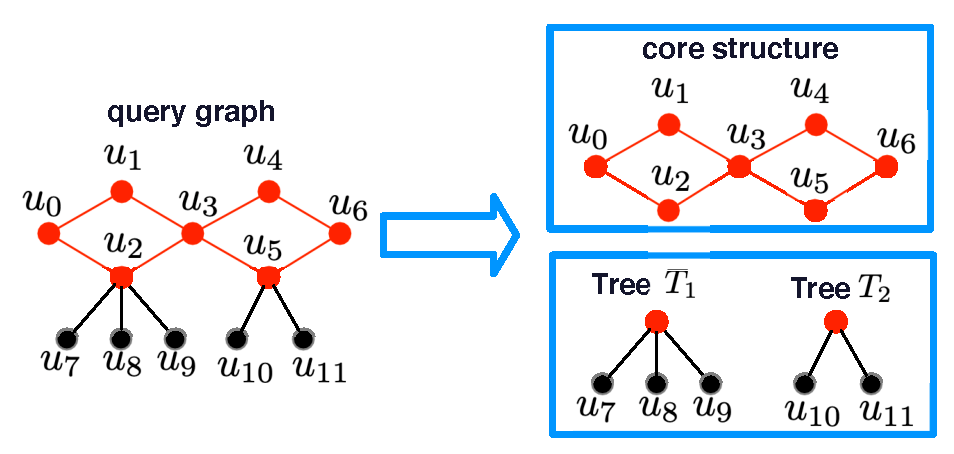
\includegraphics[width=\columnwidth]{./figure/genmatchorder.eps}
\caption{An illustration of how to decompose a query graph into a core structure and trees.}
\label{fig:matchorder}
\end{figure}
\RV{In this section, we first give a brief description of matching order generation method used in \cite{bi2016efficient}, and then demonstrate the details of our matching order generation algorithm based on NV-ext method.}

\RV{The main goal of \cite{bi2016efficient} is to match backward edges as soon as possible to eliminate invalid embeddings at early stages. Therefore, they generate a subgraph of $q$ that contains all backward edges regarding any spanning tree of $q$ by iteratively removing all degree-one vertices from $q$. The generated subgraph, which is called the core structure as shown in Figure \ref{fig:matchorder}, is matched first. In our approach, we also match the core structure first, and then the trees}.

\RV{When decomposing the core structure into extension and elimination phases, we need to adhere to an important constraint, which is that only extension patterns 0-4 can be used to decompose the core structure. The reason is explained as follows. In order to eliminate invalid embeddings as soon as possible, we need to first match circles in the core structure, which are \{$u_0$, $u_1$, $u_2$\} and \{$u_2$, $u_3$, $u_4$, $u_5$\} in Figure \ref{fig:matchorder}. Therefore, we need to extend at most two vertices when matching a circle because vertices have exactly two neighbors in a circle.}

\RV{For the core structure in Figure \ref{fig:matchorder}, we first use extension pattern 1 to match $u_0$, $u_1$, and $u_2$, then match the backward edge $(u_0, u_1)$. If we first match $u_0$, $u_1$, $u_2$, $u_4$, and $u_5$ with extension pattern 5, and then the backward edge $(u_0, u_1)$, a large number of invalid embeddings may be generated after matching the extension pattern 5, which significantly slows down the matching performance. After matching the core structure, we can use any appropriate extension patters to match trees. For example, extension patterns 5 and 1 can be used to match $T_1$ and $T_2$ in Figure \ref{fig:matchorder} respectively.}

%Many previous researches \cite{bi2016efficient,sun2020subgraph,sun2020rapidmatch,guo2020gpu} have explored how to generate an effective matching order to speed up the matching process. However, all of these methods are designed for single-vertex extension subgraph matching and not suitable for our DV-ext method. In this work, we propose a matching order generation algorithm based on the structural information of the query graph. The key idea of our algorithm is to match all available backward edges in the query graph as soon as possible to eliminate invalid partial embeddings at early stages. If no backward edges are available, we extend the partial query graph by one or two vertices. Algorithm \ref{algo:genmatchorder} demonstrates our matching order generation algorithm.
%When extending an edge that connects two matched query vertices, we can add a restriction on two matched query vertices, which is that the neighbors of one vertex must contain the other vertex. Thus, we can guarantee that the number of generated embeddings is less than or equal to the number of previous embeddings. Based on this observation,


\RV{Based on \cite{bi2016efficient} and our NV-ext method, we design Algorithm \ref{algo:genmatchorder} to generate matching order of query phases.} At the beginning of Algorithm \ref{algo:genmatchorder}, we adopt methods proposed in \cite{shi2020graphpi,mawhirter2019graphzero} to generate restrictions on VIDs in partial embeddings (line 1). Thus, we can avoid generating invalid partial embeddings. Then we generate the core structure $C$ of $q$ by iteratively removing degree-one vertices from $q$, and construct trees $T$ of $q$ using removed vertices (line 2).

In order to match the core structure (line 3), we first find the smallest circle in core structure.

The initial query phase is slightly different from the normal extension phase. In the initial phase, we match up to three query vertices in one GPU kernel, thus restricting the type of the initial phase to extension patterns 1 and 3 which have only one source vertex (lines 2-4). Different from the normal extension phase that fetches source vertices from partial embeddings, the initial phase fetches the source vertex from the edge label partition. Except for the differences, the initial phase uses the same method as the extension phase to generate partial embeddings based on the extension pattern. If no extension patterns are available for the initial phase, we choose the SV-phase that has the most neighbors (lines 5-8).

After generating the initial phase, we iteratively construct query phases for the rest vertices and edges in $q$ (line 10). First, we find all backward edges (line 11) and group them by the edge label (line 12). For each group, we construct an elimination phase (lines 13-15). If no backward edges are found, we search for two unmatched query vertices that can form one of extension patterns 1-4 (line 16). Since more than one extension patterns may be found, we assign each extension pattern a priority and choose the extension pattern with the highest priority.
\begin{itemize}
  \item Assign the first priority to extension pattern 1. As $u_1$ and $u_2$ in extension 1 have the same vertex label and source vertex, candidate sets of both vertices are equal. Therefore we can generate new embeddings of extension pattern 1 efficiently with Algorithm \ref{algo:optDV}.
  \item Assign the second priority to extension pattern 3. The candidate sets of $u_1$ and $u_2$ in extension pattern 3 are different but all belong to the neighbors of the same source vertex. Therefore, we only need to find the address of neighbors of the source vertex once and then find addresses of two vertex labels.
  \item Assign the third priority to extension pattern 4. We need to find addresses of neighbors of two source vertices and then find addresses of two vertex labels in the corresponding neighbors. Moreover, the vertex labels of $u_1$ and $u_2$ are different, this pattern will not generate invalid embeddings.
  \item Assign the fourth priority to extension pattern 2. We need to find addresses of neighbors of two source vertices and then find addresses of two vertex labels in the corresponding neighbors. As the vertex labels of $u_1$ and $u_2$ are the same, there may be same vertices in both candidate sets which can lead to invalid embeddings.
\end{itemize}

 The main issue is that there may be more than one pairs of $u_1$ and $u_2$ can form the same extension pattern with the highest priority (line 17). In our approach, we choose the pair that has the most unmatched neighbors in the query graph (line 18). In this way we increase the chance to find backward edges and high priority extension patterns when constructing the next query phase.
 %Methods proposed in \cite{guo2020gpu, shi2020graphpi,bi2016efficient} use data graph information to assist the matching order generation. We leave this method for our future work.
 If no extension patterns are found, we just select the SV-phase with the most unmatched neighbors in the query graph (lines 22-26).

\begin{algorithm}
	\KwIn{the query graph $q$}
	\KwOut{the match phase queue $matchPhase$}
	Generate restrictions to eliminate automorphisms\;
	Generate the core structure $C$ and trees $T$ of $q$\;
	Find the smallest circle $minc$ in $C$\;
%	\If{there exists EP 1 or EP 3 in $q$}{
%		Construct an initial phase $initPhase$ with the founded EP\;
%		$matchPhase.append(initPhase)$\;
%	}
%	\Else{
%		Find a pair of connected vertices that have the most neighbors in $q$\;
%		Construct an initial phase $initPhase$ with the founded pair\;
%		$matchPhase.append(initPhase)$\;
%	}
%	Delete added vertices from $q$\;
	\While{$C \neq \emptyset$}{
		\If{there are backward edges}{
			Group all backward edges by the edge label, denoted as $G$\;
			\ForEach{$g \in G$}{
				Construct an elimination phase $eliPhase$ based on $g$\;
				$matchPhase.append(eliPhase)$\;
			}	
		}
		\ElseIf{there are pairs of unmatched vertices can form one of EPs 1-4}{
			Choose the pairs whose corresponding EP has the highest priority\;
			In the chosen pairs, choose the pair that has the most neighbors\;
			Construct an extension phase $extPhase$ with the chosen pair\;
			$matchPhase.append(extPhase)$\;
			Delete added vertices from $q$\;
		}
		\Else{
			Find a pair of connected vertices that have the most neighbors in $q$\;
			Construct an extension phase $extPhase$ with the founded pair\;
			$matchPhase.append(extPhase)$\;
			Delete added vertices from $q$\;
		}
	}
	
	\caption{genMatchOrder}
	\label{algo:genmatchorder}
\end{algorithm}

\subsection{Load Balance}
In GPU, once a thread block is scheduled to run on an SM, it will not be scheduled out until all warps in this thread block are finished. Therefore, if one warp matches a vertex or an edge that has many candidates, all warps in the same thread block have to wait for its completion. To address this problem, GSI designs a four-layer balance scheme. However, their scheme needs to invoke a GPU kernel inside a GPU kernel, which is time-consuming as illustrated in Section \ref{sec:compargsi}. Different from GSI, we use fixed warps, which means the maximum concurrent warps are generated and will not be scheduled out during execution, to perform subgraph matching. In this way, a warp with small workload can match next embedding without waiting for other warps. Only when there is no embeddings left, the faster warps have to wait for the slower warps. Our approach is simple yet effective, it can mitigate load imbalance to some extend. A more powerful load balance scheme can be designed and we leave this for a future study. 